%%%%%%%%%%%%%%%%%%%%%%%%%%%%%%%%%%%%%%%%%
% Wenneker Assignment
% LaTeX Template
% Version 2.0 (12/1/2019)
%
% This template originates from:
% http://www.LaTeXTemplates.com
%
% Authors:
% Vel (vel@LaTeXTemplates.com)
% Frits Wenneker
%
% License:
% CC BY-NC-SA 3.0 (http://creativecommons.org/licenses/by-nc-sa/3.0/)
% 
%%%%%%%%%%%%%%%%%%%%%%%%%%%%%%%%%%%%%%%%%

%----------------------------------------------------------------------------------------
%	PACKAGES AND OTHER DOCUMENT CONFIGURATIONS
%----------------------------------------------------------------------------------------

\documentclass[11pt]{scrartcl} % Font size

%%%%%%%%%%%%%%%%%%%%%%%%%%%%%%%%%%%%%%%%%
% Wenneker Assignment
% Structure Specification File
% Version 2.0 (12/1/2019)
%
% This template originates from:
% http://www.LaTeXTemplates.com
%
% Authors:
% Vel (vel@LaTeXTemplates.com)
% Frits Wenneker
%
% License:
% CC BY-NC-SA 3.0 (http://creativecommons.org/licenses/by-nc-sa/3.0/)
% 
%%%%%%%%%%%%%%%%%%%%%%%%%%%%%%%%%%%%%%%%%

%----------------------------------------------------------------------------------------
%	PACKAGES AND OTHER DOCUMENT CONFIGURATIONS
%----------------------------------------------------------------------------------------

\usepackage{amsmath, amsfonts, amsthm} % Math packages

\usepackage{listings} % Code listings, with syntax highlighting

\usepackage[main = greek, english]{babel} % English language hyphenation

\usepackage{graphicx} % Required for inserting images
\graphicspath{{Figures/}{./}} % Specifies where to look for included images (trailing slash required)

\usepackage{booktabs} % Required for better horizontal rules in tables

\usepackage{dirtytalk} % Required for quoting.

\usepackage{float} % Added for hard placement of images.

\usepackage[dvipsnames]{xcolor} % Added for extra colors.

\usepackage{tikz} % For colored boxes and more.

\numberwithin{equation}{section} % Number equations within sections (i.e. 1.1, 1.2, 2.1, 2.2 instead of 1, 2, 3, 4)
\numberwithin{figure}{section} % Number figures within sections (i.e. 1.1, 1.2, 2.1, 2.2 instead of 1, 2, 3, 4)
\numberwithin{table}{section} % Number tables within sections (i.e. 1.1, 1.2, 2.1, 2.2 instead of 1, 2, 3, 4)

\usepackage{enumitem} % Required for list customisation
\setlist{noitemsep} % No spacing between list items

%----------------------------------------------------------------------------------------
%	DOCUMENT MARGINS
%----------------------------------------------------------------------------------------

\usepackage{geometry} % Required for adjusting page dimensions and margins

\geometry{
	paper=a4paper, % Paper size, change to letterpaper for US letter size
	top=2.5cm, % Top margin
	bottom=3cm, % Bottom margin
	left=3cm, % Left margin
	right=3cm, % Right margin
	headheight=0.75cm, % Header height
	footskip=1.5cm, % Space from the bottom margin to the baseline of the footer
	headsep=0.75cm, % Space from the top margin to the baseline of the header
	%showframe, % Uncomment to show how the type block is set on the page
}

%----------------------------------------------------------------------------------------
%	FONTS
%----------------------------------------------------------------------------------------

\usepackage[utf8]{inputenc} % Required for inputting international characters
\usepackage[T1]{fontenc} % Use 8-bit encoding

%----------------------------------------------------------------------------------------
%	SECTION TITLES
%----------------------------------------------------------------------------------------

\usepackage{sectsty} % Allows customising section commands

\sectionfont{\vspace{6pt}\centering\normalfont\scshape} % \section{} styling
\subsectionfont{\normalfont\bfseries} % \subsection{} styling
\subsubsectionfont{\normalfont\itshape} % \subsubsection{} styling
\paragraphfont{\normalfont\scshape} % \paragraph{} styling

%----------------------------------------------------------------------------------------
%	HEADERS AND FOOTERS
%----------------------------------------------------------------------------------------

\usepackage{scrlayer-scrpage} % Required for customising headers and footers

\ohead*{} % Right header
\ihead*{} % Left header
\chead*{} % Centre header

\ofoot*{} % Right footer
\ifoot*{} % Left footer
\cfoot*{\pagemark} % Centre footer

\newcommand{\img}[1]
{
    \begin{center}
        \fcolorbox{black}{white}{\includegraphics[height=10em]{#1}}
    \end{center}

}

% Helper Macros

\newcommand{\en}[1]{\foreignlanguage{english}{#1}}
\newcommand{\src}[1]{{\ttfamily\en{#1}}}


% Extra Formatting

\setlength{\parindent}{0em}
\setlength{\parskip}{1em}
 % Include the file specifying the document structure and custom commands

\usepackage{subcaption}
\usepackage{amsmath}

%----------------------------------------------------------------------------------------
%	TITLE SECTION
%----------------------------------------------------------------------------------------

\title{	
	\normalfont\normalsize
	\textsc{Πανεπιστήμιο Πατρών, Τμήμα Ηλεκτρολόγων Μηχανικών και Τεχνολογίας Υπολογιστών}\\ % Your university, school and/or department name(s)
	\vspace{25pt} % Whitespace
	\rule{\linewidth}{0.5pt}\\ % Thin top horizontal rule
	\vspace{20pt} % Whitespace
	{\Large Εργασία: \en{Pokemon}}\\ % The assignment title
	\vspace{12pt} % Whitespace
	\rule{\linewidth}{2pt}\\ % Thick bottom horizontal rule
	\vspace{12pt} % Whitespace
}

\author{\LARGE Ευάγγελος Λάμπρου \\ \en{UP1066519}} % Your name

\date{} % Today's date (\today) or a custom date

\begin{document}

\maketitle 

\tableofcontents

\newpage

\section{Εισαγωγή}

\section{Ερωτήματα Εργασίας}

\subsection{\en{Explain briefly in your own words tasks 1-3.}}
\subsubsection{\en{Cube simulation.}}

Μπορούμε για την προσομοίωση του κύβου να ορίσουμε παραμέτρους όπως η αρχική του θέση, ταχύτητα, 
γωνιακή ταχύτητα, μάζα και μήκος. 

Ενεργοποιώντας την χρήση \en{quaternions}, παρατηρούμε διαφορετική συμπεριφορά του κύβου ως προς την περιστροφή του.

\begin{figure}[H]
	\begin{center}
		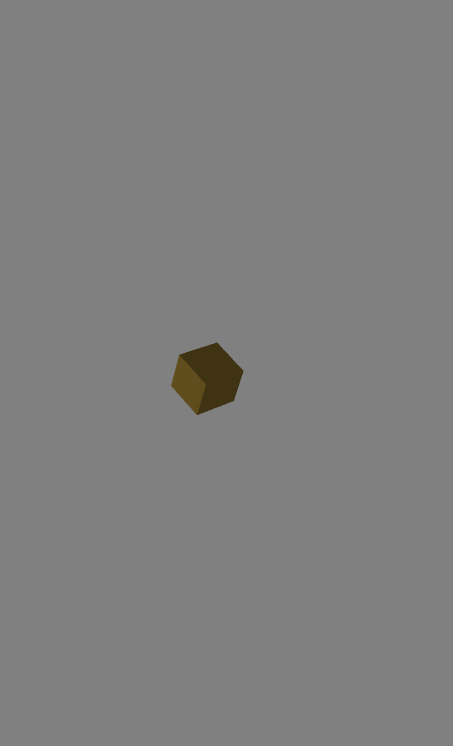
\includegraphics[height=.5\textheight]{./assets/cube.png}
	\end{center}
	\caption{Ο κύβος να περιστρέφεται}
\end{figure}

\subsubsection{\en{Simulation of a sphere.}}

Μετά από μία σύγκρουση, η ταχύτητα της σφαίρας θα είναι με βάση τον τύπο:

\begin{equation}
	\vec{v}^\prime = v - 2 \cdot (\vec{v} \cdot \vec{n}) \cdot \vec{n}	
\end{equation}

Όπου $\vec{n}$ είναι η κατεύθυνση της σύγκρουσης.

Για να πρσθέσουμε τη δύναμη της βαρύτητας στην προσομοίωσή μας αρκεί να εφαρμόσουμε στη σφαίρα 
μία δύναμη $F = -m \cdot g$ στην κατεύθυνση του άξονα $y$.
Παρατηρούμε πως όσο αναπηδάει η σφαίρα στον κύβο, το ύψος της όλο και αυξάνεται. 
Αυτό οφείλεται στο σφάλμα της προσομοίωσης το οποίο προσθέτει στην ολική ενέργεια της σφαίρας.

Θέτοντας το $dt = 0.001$ η προσομοίωση κυλάει πλέον με πολύ πιο αργό ρυθμό (ο ρυθμός αυτός 
εξαρτάται και από το \en{framerate} της εφαρμογής μας). Αλλάζοντας τη μέθοδο ολοκλήρωσης 
από την \en{Euler} στην \en{Runge-Kutta 4th Order} βλέπουμε πως το σφάλμα, άρα και η ολική 
ενέργεια της σφαίρας αυξάνονται με πιο αργό ρυθμό.

\begin{figure}[H]
	\begin{center}
		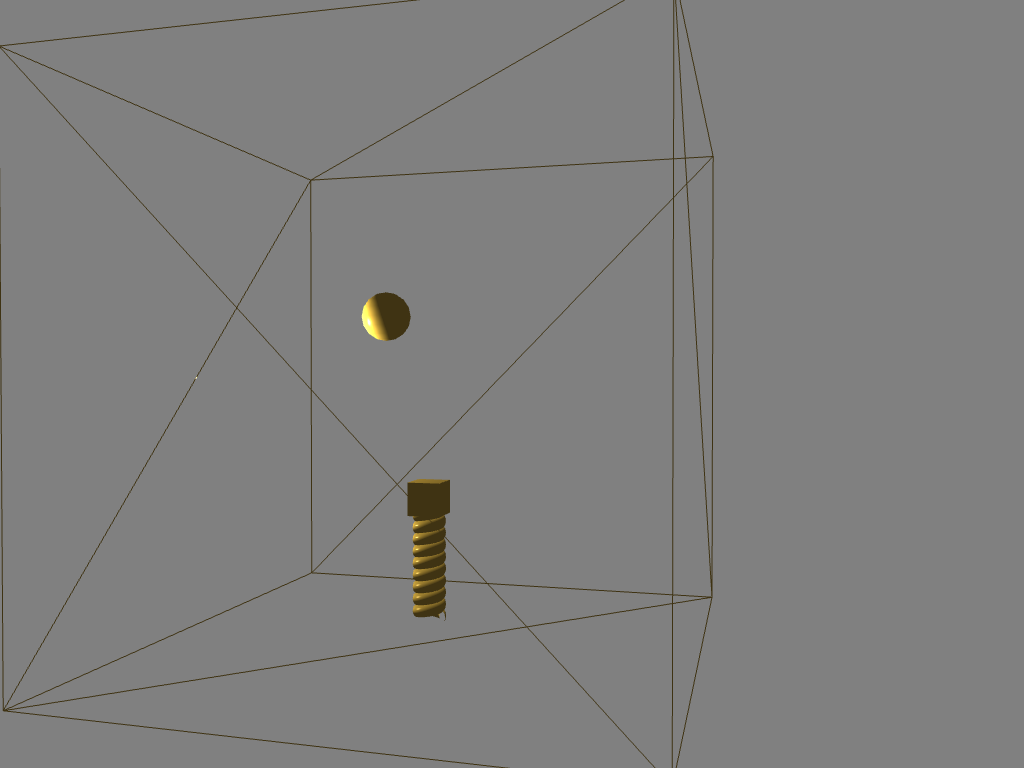
\includegraphics[height=.5\textheight]{./assets/ball.png}
	\end{center}
	\caption{Η σφαίρα να αναπηδάει στα τοιχώματα του μεγαλύτερου κύβου ενώ της ασκείται δύναμη από τη βαρύτητα.}
\end{figure}

\subsubsection{\en{Model a mass-spring damper system.}}

Για να μοντελοποιήσουμε το σύστημα μάζας ελατηρίου αρκεί να εφαρμόσουμε σε ένα 
\en{rigid body} (το αντικείμενο που θα ταλαντώνεται) μία δύναμη της μορφής:

\begin{equation}
	\Sigma F = -k \cdot (x - l_0) + m \cdot g - b \cdot x	
\end{equation}

Μπορούμε για το σύστημα να ορίσουμε τις παραμέτρους $k$ (σκληρότητα ελατηρίου), $l_0$ (μήκος παραμόρφωσης σε ηρεμία), 
$b$ (συντελεστής απόσβεσης ταλάντωσης).
Ακόμα μπορούμε να αλλάξουμε τις αρχικές συνθήκες του συστήματος όπως η αρχική ταχύτητα, θέση και μάζα του ταλαντευόμενου σώματος.

\begin{figure}[H]
	\begin{center}
		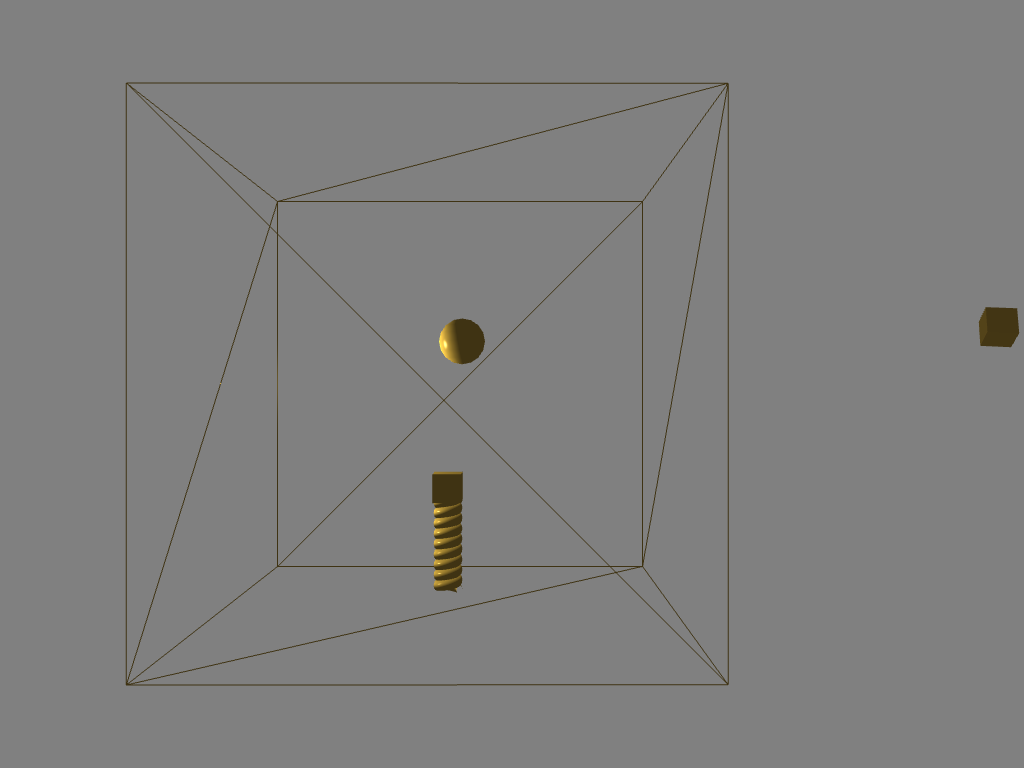
\includegraphics[height=.5\textheight]{./assets/spring.png}
	\end{center}
	\caption{Η προσομοίωση του συστήματος μάζας-ελατηρίου.}
\end{figure}

\subsection{\en{Generate three or more balls with different masses and radii and 
have them all interact with the box and with each other.}}

Προσθέτουμε πολλές σφαίρες σε ένα \en{std::vector}. Έπειτα, κάνουμε για κάθε σφαίρα ελέγχους σύγκρουσης με τον περιβάλοντα κύβο, όπως
και με όλες τις άλλες σφαίρες. 

Ο έλεγχος επαφής σφαίρα με σφαίρα γίνεται με βάση τον τύπο: 

\begin{equation}
	||\vec{p_1} - \vec{p_2}|| < r_1 + r_2
\end{equation}

Όπου η $\vec{p_i}, r_i$ η θέση και ακτίνα της κάθε σφαίρας αντίστοιχα.

\begin{figure}[H]
	\begin{center}
		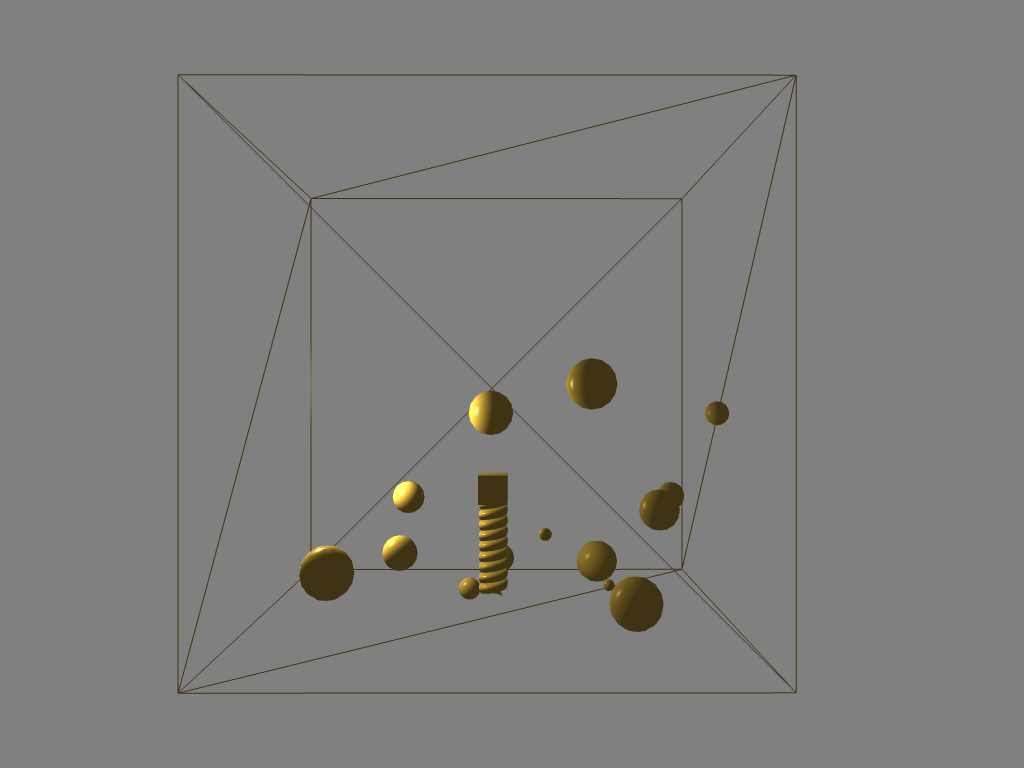
\includegraphics[height=.5\textheight]{./assets/ballz.png}
	\end{center}
	\caption{Η προσομοίωση πολλών αλληλεπιδρώντων σφαιρών.}
\end{figure}

\end{document}
